\documentclass[12pt,a4paper,openright]{report}
\usepackage[utf8]{inputenc}
\author{ABELARD Jérémy}
\usepackage[T1]{fontenc}
\usepackage[a4paper,left=2.5cm,right=2.5cm,top=2cm,bottom=2cm]{geometry}
\usepackage[french]{babel}
\AddThinSpaceBeforeFootnotes
\FrenchFootnotes
\usepackage{xspace}
%\usepackage{microtype} %éviter au max les césures
\usepackage{hyperref}
\usepackage{mathptmx}
\usepackage[pdftex]{graphicx}
\usepackage{amsmath}
\renewcommand*{\overrightarrow}[1]{\vbox{\halign{##\cr 
  \tiny\rightarrowfill\cr\noalign{\nointerlineskip\vskip1pt} 
  $#1\mskip2mu$\cr}}}
\usepackage{amsfonts}
\usepackage{textcomp}
\usepackage{amssymb}
\usepackage{makeidx}
\usepackage{fancyhdr}
\usepackage{caption}
\usepackage{float}
\usepackage{subcaption}
\usepackage{array}
\usepackage{setspace}
\usepackage{xcolor}
\usepackage{colortbl}%Coloration tableau
\usepackage[bottom,flushmargin,hang,multiple]{footmisc}
%\usepackage{nomencl}
%\makenomenclature
\setlength{\parindent}{1cm}
\setlength{\parskip}{1ex plus 0.5ex minus 0.2ex}
\newcommand{\hsp}{\hspace{20pt}}
\newcommand{\HRule}{\rule{\linewidth}{1.5mm}}
\pagestyle{fancy}
\lhead{}%haut de page gauche
\chead{}%haut de page centre
\rhead{}%haut de page droite
\lfoot{}%pied de page gauche
\cfoot{\thepage}%pied de page centré
\rfoot{}%pied de page droit
\renewcommand{\headrulewidth}{1pt}
\renewcommand{\footrulewidth}{1pt}
\onehalfspacing %Interlignes 1.5cm
\renewcommand{\thesection}{\arabic{section}} 

\begin{document}
 \begin{titlepage}
  \begin{figure}
   \begin{center}
     
\includegraphics[scale=0.1]{UR}
     \hspace{1.8cm}
     
\includegraphics[scale=0.8]{logoFST}
  
   \end{center}
   \begin{center}
   %{ \huge \textit{\bfseries Mini-projet : \\[0.4cm] }}
   
%arrangement de la page de garde 
    \title{\vspace{3cm} %emplacement du titre principal
    
%tout ce qui vont autour
   
  
    \textrm{\Large Stage en laboratoire}\\[2cm]
    {\hrule {\vspace{1cm}
     \textbf{Optimisation de l'inclinaison et l'orientation d'un panneau solaire à La Réunion}}
    \\[1cm]
    \hrule {\vspace{0.4cm}}}
    
     {\slshape Encadrant : Professeur Miloud Bessafi}\\[1cm]
     
\includegraphics[scale=0.2]{le2p_fondtrans}
     {\vspace{3cm}}   }%{une image en relation avec le rapport}
    
    
    %{\vspace{3cm}\textit{Par :}\\ ABELARD Jérémy} % peut être remplacer par l'auteur
    %vspace{3cm}\\
   	%Année universitaire : 2019 - 2020
   	%}}
   
 \maketitle %date généré
  		
   \end{center}
 
  \end{figure}
     
 \end{titlepage}

\chapter*{Remerciement}
\begin{center}
Je tiens à remercier mon encadrant de stage le \textbf{Pr. Bessafi Miloud} pour son investissement en tant qu'encadrant mais aussi en tant que professeur.

Je tiens aussi à remercier \textbf{Mme Morel Béatrice} et \textbf{Mr Benne Michel} qui sont les professeurs pédagogiques du Master 1 \& 2 Énergie, pour avoir permis aux étudiants d'avoir un sujet de stage en vue de la crise sanitaire lier au COVID-19.
\end{center}
	\renewcommand{\contentsname}{Sommaire}
	\tableofcontents
	\newpage
	
\section*{Introduction}
	\addcontentsline{toc}{section}{Introduction}

Ce rapport décrit le stage effectuait en M1 Énergie au laboratoire Energie-Lab (LE2P) à l'université de La Réunion. En vue de la crise sanitaire que traverse le pays le laboratoire Energy-Lab à proposer aux étudiants de Master des sujets de stage en lien avec leur formation. L'objectif du stage prend en compte la mise en place du confinement et oriente les projets vers des outils de programmation. L'intituler de ce rapport est : \textbf{optimisation de l'inclinaison et l'orientation d'un panneau solaire à La Réunion}. 

Le but est, dans un premier temps, de travailler sur des modèles de solarimétrie pour une année type (ici 2005) pour 5 stations dans  l'ensemble de l'île : Nord, Sud, Est, Ouest et Centre. Dans un second temps, il est demandé de calculer le facteur de transposition pour chaque station, ce qui implique alors l'étude de différents paramètres et la mise en place d'un protocole expérimentale. Ceci permettra de calculer le facteur de transposition.

 La lecture des données solaire en masse requiert forcément l'utilisation d'un logiciel de programmation, pour faciliter la lecture et le calcule du facteur de transposition. 

Ce rapport se déroule comme suit: 
tout d'abord une visualisation globale du type de données traitées, ainsi que la méthodologie mise en place. Ce qui apportera par la suite la visualisation des résultats obtenue, et pour finir la dernière partie sera consacrée à la discussion de ces résultats.

\newpage
\section{Présentation de l'entreprise}
Le stage s'effectue dans le laboratoire Energie-Lab anciennement appelé LE2P (Laboratoire d'Energétique, d'Electronique et de Procédés) est dirigé par Jean-Pierre Chabriat. Créé en 2006, il contient une équipe d'accueil au sein de la Faculté des Sciences et Technologies à l'Université de la Réunion. Cette équipe contient des chercheurs en énergétique et électronique ; ciblant la télécommunication et la physique de l'environnement.
Le laboratoire possède 3 opérations scientifiques "OS" qui possède un axe de recherche commun : L'optimisation de systèmes énergétiques solaires ou intermittents intelligents.
Les 3 opérations scientifiques sont les suivantes :
\begin{itemize}
\item OS 1 Gisement Solaire : variabilité à La Réunion et en zone tropicale, métrologie et modélisation.
\item OS 2 Stockage et conversion de l’énergie : systèmes PAC et hybridation.
\item OS 3 Optimisation énergétique des réseaux de capteurs WSN.
\end{itemize}
Le stage que j'ai effectué fait partie de l'OS 1 qui s'oriente sur l'application de la  prévisibilité des changements climatiques et des variations journalières et horaires. Le but était de documenter sur la variabilité du rayonnement solaire incident à la surface, particulièrement dans la zone sud-ouest de l'océan Indien. Pour ce faire, il faut avoir des données de rayonnement de haute résolution ainsi qu'une zone spatiale et temporelle prélevant des données en continu.

L'OS 1 se concentre principalement sur la caractérisation d'une source d'énergie renouvelable qui est le rayonnement solaire et la modélisation énergétique de systèmes utilisant une source intermittente qui varie dans l'espace et le temps.

\section{Données, modèle et méthodologie}
\subsection{Le modèle d'étude}

En vue du sujet de stage qui a été énoncer dans l'intituler de ce rapport, le prélèvement des données se fera sur le territoire réunionnais. Les liens suivants nous dirigent vers des bases de données relatives à notre étude :
\begin{itemize}
\item SoDa "\textbf{SO}lar radiation \textbf{DA}ta": \url{http://www.soda-pro.com/web-services/radiation/helioclim-3-archives-for-free}
\item SOLPOS "\textbf{SOL}ar \textbf{POS}ition and Intensity: \url{https://midcdmz.nrel.gov/solpos/solpos.html}
\end{itemize}

\noindent Le premier lien concerne des données météorologiques et de radiation, où seulement le rayonnement global sera étudié dans ce projet. Le deuxième concerne des données de course solaire.
\newpage
Le facteur de transposition dépend de la zone géographique que l'on souhaite étudier. Selon l'endroit où l'on effectue l'étude, nous pourrons déduire l'orientation et l'inclinaison du panneau afin d'avoir une meilleure optimisation. Le schéma ci-après explique le contexte d'étude: 

\begin{figure}[h!]
  \begin{center}
    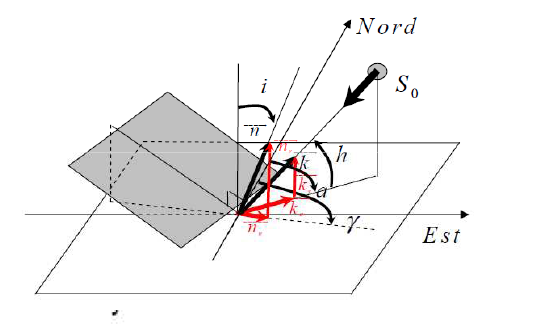
\includegraphics[scale=0.8]{coursesolaire}
    \caption{Visualisation du système d'étude}
  \end{center}
\end{figure}

\noindent Une description s'impose:

\begin{itemize}
\item $\vec{n}$ : vecteur normal au panneau et ses composantes $\overrightarrow{n_H}$ et $\overrightarrow{n_V}$.
\item $\vec{k}$ : vecteur sur l'axe panneau-soleil et ses composantes $\overrightarrow{k_H}$ et $\overrightarrow{k_V}$.
\item $i$ : angle d'inclinaison du panneau, quand $i$ = 0° le panneau est horizontale.
\item $\gamma$ : angle d'orientation du panneau.
\item $a$ : angle solaire azimut, en prenant le Sud = 0°.
\item $h$ : angle d'élévation du soleil obtenu en inversant l'angle du zénith.
\end{itemize}

Nous allons un peu plus loin en entamant l'étude théorique du facteur de transposition et en associant les différents paramètres vus précédemment.

\subsubsection{Partie théorique}

\noindent Le calcule du facteur de transposition (FT) est sous la forme suivante :

$FT = \frac{\textit{Rayonnement Global cumulé annuel reçu sur le panneau orienté}}{\textit{Rayonnement Global cumulé annuel reçu sur le panneau horizontal}}$

\noindent Le facteur de transposition implique alors le calcule du rayonnement global cumulé pendant une année.
Il va falloir alors calculer ce rayonnement global G* pour ainsi calculer le facteur de transposition :

\begin{center}
$FT = \frac{\sum_{p=1}^N G^*(i,\gamma,a(t_p),h(t_p))}{\sum_{p=1}^N G^*(0,\gamma,a(t_p),h(t_p)}$
\end{center}

\begin{figure}[h!]
  \begin{center}
    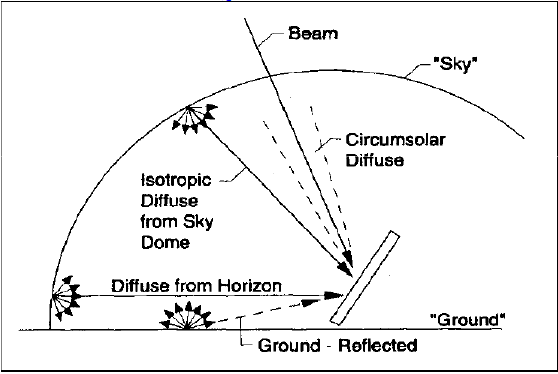
\includegraphics[scale=0.5]{diffrayonn}
    \caption{Les différents rayonnements nécessaire au calcule du facteur de transposition.}
  \end{center}
\end{figure}
\newpage
\noindent Le calcule du rayonnement solaire est donné par l'équation de l'éclairement solaire indiqué dans l'\textbf{annexe A} :

\begin{itemize}
\item \textbf{Rayonnement global, $G^*=S^*+D^*$}: 
	\begin{equation}
	FT = \frac{\sum_{p=1}^N S^*(i,\gamma,a(t_p),h(t_p))+ D^*(i)}{\sum_{p=1}^N S^*(0,\gamma,a(t_p),h(t_p)+ D^*(0)}
	\end{equation}	 
	
\item \textbf{S* rayonnement direct} :\\
$S^*(i,\gamma,a(t_p),h(t_p))= S_0.(\vec{k}\bullet\vec{n})$\\
\noindent \underline{Avec} :\\
$(\vec{k}\bullet\vec{n}) \left\{
    \begin{array}{ll}
        \ \vec{k}=\vec{k_V}+\vec{k_H} \\
        \ \vec{n}= \vec{n_V} + \vec{n_H}
    \end{array}
\right. $\\
\\
\underline{En calculant le produit scalaire on obtient} :\\
$(\vec{k}\bullet\vec{n})= (cos(h).sin(i).cos(\gamma - a) + sin(h).cos(i))$\\

\underline {On obtient alors} :
	\begin{equation}
	S^*(i,\gamma,a(t_p),h(t_p))= S_0.(cos(h).sin(i).cos(\gamma - a) + sin(h).cos(i))
	\end{equation}
	Si $i=0$ ; $S^*(0,\gamma,a(t_p),h(t_p))=S_0.sin(h)$\\
	
\item \textbf{D* rayonnement diffus} :\\
Le rayonnement diffus est obtenu par la somme du rayonnement diffus provenant du ciel (aérosol, nuage, atmosphère...) et du rayonnement diffus obtenue au sol, $D^* = D_{ciel} + D_{sol}$ (cf. \textbf{Figure 2}).

 	\begin{equation}
D^*(i) = \left(\frac{1+cos(i)}{2}\right)D_h + \alpha\left(\frac{1-cos(i)}{2}\right)\left(D_h + S_0.sin(h)\right)
	\end{equation}
	Si $i=0$ ; $D^*(0)= D_h$
\end{itemize}
\newpage
Comprendre la partie théorique permet déjà de connaître les différents paramètres qui faudra prendre en compte lors de l'encodage. De là, les étapes de programmation sera établie pour parvenir à l'objectif fixé sans se mêler les pinceaux.

\subsection{Les données}
Après la partie théorique faite, il faudra récolter les données solaires.
%Site Helio clim explication...(mettre en annexe)
Premièrement sur le site web SoDa dans la base de données \href{http://www.soda-pro.com/web-services/radiation/helioclim-3-archives-for-free}{\textcolor{blue}{\underline{Helioclim-3}}}, sera collecter des données météorologiques où seulement le rayonnement global nous intéressera. Les prélèvements de ces données sont mensuels et non annuels afin de réduire le temps de téléchargement. Ces données concernent l'année 2005 et les 5 secteurs sont les suivantes :

\begin{enumerate}
\item \textit{Nord}: Gillot, Saint-Denis (lat.-20,9;long.55,5)
\item \textit{Ouest}: Saint-Leu (lat.-21,163;long.55,326)
\item \textit{Sud}: Saint-Joseph (lat.-21,335;long.55,612)
\item \textit{Est}: Saint-Benoît (lat.-21,1;long.55,7)
\item \textit{Centre}: Le Tampon (lat.-21,2;long.55,571)
\end{enumerate}

%site Solpos (annexe) décrire le site brièvement.
Ensuite, nous avons les données de course solaire qui seront prélevées parallèlement aux données de rayonnement solaire. Le site web \href{https://midcdmz.nrel.gov/solpos/solpos.html}{\textcolor{blue}{\underline{SOLPOS}}} possède une base de données de course solaire,  les données qui seront prises en compte dans ce projet sont des données d'angle azimut et zénith. 

\textbf{\underline{NB}}: l'angle d'azimut vaut 0° au Nord sur SOLPOS alors qu'on souhaite avoir un angle de 0° au Sud. Les équations vues précédemment sont calculées de telle sorte à prend en compte l'axe du Sud qui vaut 0°. Il faudra alors prendre en compte la conversion de l'azimut dans l'encodage du facteur de transposition (FT).

\begin{figure}[h!]
\begin{center}
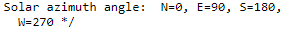
\includegraphics[scale=1]{refAzimuth}
\caption{Angle de référence pour l'azimut sur SOLPOS.}
\end{center}
\end{figure}

%passer à l'explicatiion des diapositives (les données de référence, courbe graph...)
les graphiques qu'on obtiendra dans ce projet doivent se rapprocher plus ou moins aux graphiques donnés dans l'\textbf{annexe B}).
notre objectif est alors d'afficher ce type de graphique pour les différentes zones géographiques donner précédemment.

il ne reste plus qu'à effectuer la programmation avec ce qu'on a vu jusqu'à maintenant.

\subsubsection*{Partie programmation}
Le logiciel de programmation qui est utilisé ici est Python. Le codage du facteur transposition suit les étapes suivantes.

Premièrement il faut importer les différentes librairies pour faciliter l'encodage. Les librairies utilisées sont : Numpy et Pandas, ainsi que les librairies graphiques, Matplotlib et Seaborn.\newline
Il va falloir ensuite entrer les différentes équations pour arriver à calculer le facteur de transposition (FT).

Pour entrer des fonctions dans python, on utilise le paramètre \textit{"def"}. Cependant l'équation de FT comporte plusieurs sous équations, donc des sous fonctions à entrer dans Python. $S^*$ et $D^*$ sont ses sous fonctions, $i$, $\gamma$, $a$ et $h$ sont les variables à prendre aussi en compte.\\
\noindent Nous aurons donc la fonction principale du facteur de transposition :\\
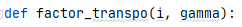
\includegraphics[scale=0.7]{deffact}\\
Avec les sous-fonctions :
\begin{itemize}
\item S* : 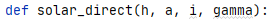
\includegraphics[scale=0.7]{defsolar}
\item D* :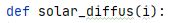
\includegraphics[scale=0.7]{defdiffus}
\end{itemize}
\medskip

Il faudra ensuite pour chaque fonction écrire l'équation qu'il doit contenir (vu en \textbf{section 1.1} Partie théorique). Ce qu'il faut noter c'est que pour appeler les fonctions trigonométriques (cos, sin, pi...) avec Numpy il faudra ajouter devant chaque fonction le paramètre "$np.$", par exemple : $np.cos()$, $np.sin()$, etc..

Par la suite, Il est logique d'appeler les Dataframes contenant nos données. Mais avant de les appeler il va falloir fusionner ces données, car les fichiers récoltés sont mensualisés et pour les calculer nous devons obtenir des données annuelles. Il va falloir fusionner dans un premier temps les fichiers d'Hélioclim et dans un deuxième temps les fichiers SOLPOS, pour ainsi avoir des fichiers correspondant à des données sur une année. Nous devons alors avoir dans le fichier Hélioclim et SOLPOS le même nombre de lignes pour qu'ils correspondent au même \textit{datetime}.

On appelle dans le programme les deux fichiers obtenus avec les variables suivantes : \textit{f1} pour le fichier SOLPOS et \textit{f2} pour le fichier Hélioclim.
% mettre les premier ligne des deux fichier pour avoir une vu d'ensemble.
\begin{figure}[h!]
\begin{center}
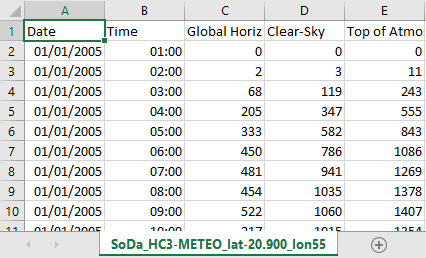
\includegraphics[scale=0.6]{tableS0}
\caption{Les premières ligne du fichier Helioclim-3.}
\end{center}
\end{figure}

\begin{figure}[h!]
\begin{center}
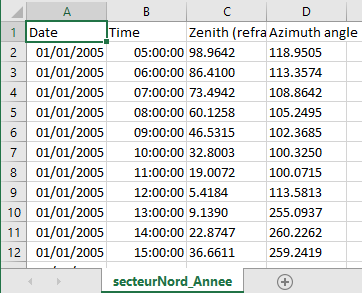
\includegraphics[scale=0.6]{tableAZI}
\caption{Les premières ligne du fichier SOLPOS.}
\end{center}
\end{figure}
\newpage
 On remarque alors que le fichier Helioclim contient des colonnes qui ne sont pas utiles à notre étude; le paramètre "$drop()$" servira à ne pas prendre en compte ces colonnes. Ce qui nous intéresse ici c'est la colonne "Global Horizon" qui correspond à la valeur de $S_0$ dans les équations.

Il y a eu des modifications qui ont été apportées au niveau de l'angle $h$ du zénith et de l'angle $a$ de l'azimut; les modifications sont telle que : pour $a$ comme vu à la \textbf{section~1.2}, il faudra effectuer une rotation sur $-\pi$ à l'angle d'azimut, pour considérer le Sud égale à 0°. Pour $h$ il faudra inverser l'angle de zénith pour avoir l'élévation.
\begin{figure}[h!]
\begin{center}
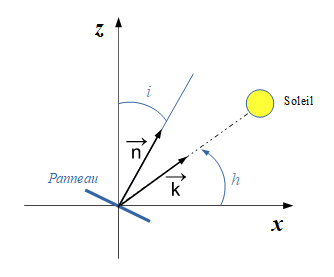
\includegraphics[scale=0.6]{coursesolaire1}
\end{center}
\end{figure}

\noindent Ensuite nous avons à coder les boucles "\textit{for}" pour les angles $i$ et $\gamma$:

\begin{figure}[h!]
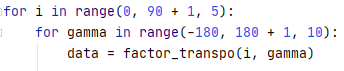
\includegraphics[scale=0.7]{bouclefor}
\end{figure}

 Le but est d'afficher le facteur de transposition (FT) pour chaque angle $i$ et $\gamma$ afin de visualiser le graphique selon ces deux angles (ex : \textbf{annexe B}). Il ne faut pas oublier la dernière boucle à effectuer, celui du temps (voir \textbf{annexe C}). Elle permettra de sommer chaque ligne $p$ comme vu dans l'équation de FT au numérateur et au dénominateur. Ce qui donnera une unique valeur FT pour un angle $i$ et $\gamma$ donné.

\textbf{\underline{NB}} : les données qui correspond aux angles sont en degrés. Avec le paramètres "\textit{np.radians}" de Numpy ces données seront automatiquement convertis en radiant. Par défaut Python effectue des calculs trigonométriques en radiant et non en degrés.

Enfin, avant de visualiser de quelconque résultat il va falloir coder le type de graphique qu'on veut faire apparaître. Le type de graphique qu'on visualisera est un "heatmap" qui est un graphique matriciel qui est à la base conçue pour visualiser l'évolution de la température en fonction de 2 paramètres. Ici nous visualiserons un diagramme matriciel qui contient trois dimensions; nous aurons alors pour axes $i$ en ordonnée, $\gamma$ en abscisse, et FT qui varie en fonction de la couleur.

Chaque fois qu'on lancera le programme un nouveau fichier sera créé. Il y aura dans ce fichier les données du facteur de transpositions pour chaque $i$ et $\gamma$. Cela permettra de visualiser ou modifier le graphique sans qu'à chaque instant on ait à relancer le programme principal qui prend beaucoup de temps à compiler.

\begin{figure}[h!]
\begin{center}
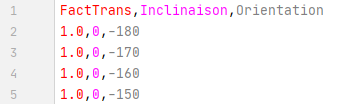
\includegraphics[scale=0.6]{dataFT}
\caption{Les premières lignes du fichier créer.}
\end{center}
\end{figure}

Ces étapes ont permis d'avoir une vue d'ensemble sur chaque paramètre à entrer dans python. Ce qui emmènera à coder au mieux le facteur de transposition. Ces étapes permettent aussi de ne rien oublier, car un seul oublie fausse totalement les résultats. Pour valider ces résultats, il suffira d'afficher les graphiques et de voir le comportement. 
%\smallskip %intervale de ligne autre medskip et bigskip

%\begin{itemize}
%\item
%\end{itemize}

%\begin{enumerate}
%\item
%\end{enumerate}

%\begin{description}
%\item[textgras] signification
%\end{description}
\newpage
\section{Résultats}
%donner resultat:S*, D*, tableau (FT, Inc et Orient),(dificulter rencontrer?) diagramme albédo, diagramme polaire.
Nous passons maintenant aux résultats. les figures suivantes permettent de comprendre l'évolution des données à chaque étape de la programmation. Visualisons dans un premier temps l'évolution du rayonnement global horizontal dans une journée, donner dans le fichier Hélioclim-3 qui représente $S_0$ :

\begin{figure}[h!]
\begin{center}
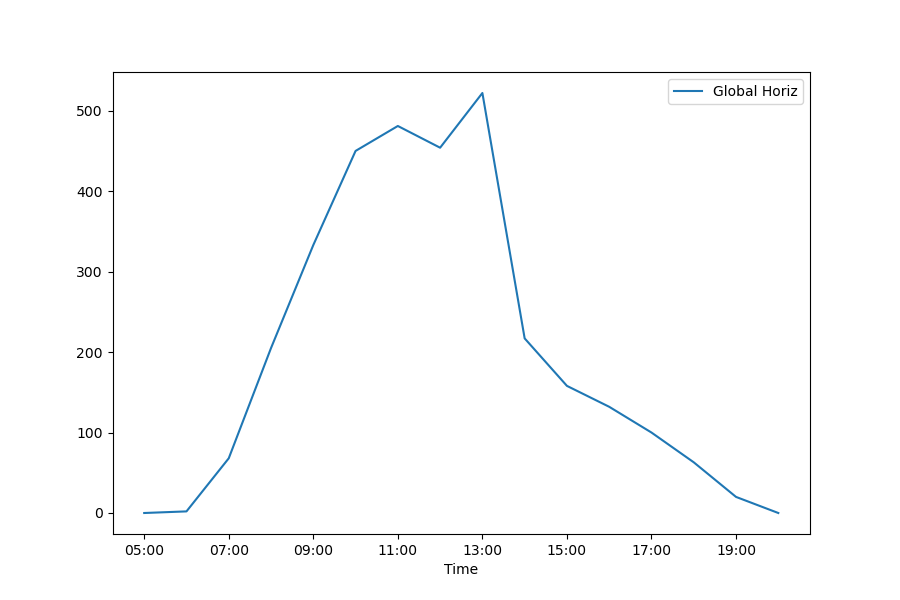
\includegraphics[scale=0.4]{figSolarglob}
\caption{Évolution de $S_0$.}
\end{center}
\end{figure}

Après calcul de S* et D* pour $i$ et $\gamma$ égale à 50° et en utilisant les données de la figure précédente on obtient les graphiques suivants :

\begin{figure}[h]
\begin{center}
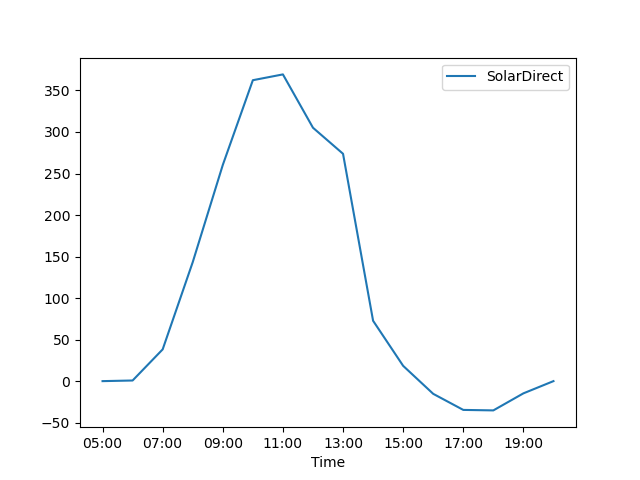
\includegraphics[scale=0.45]{figSolardirect}
\hspace{1cm}
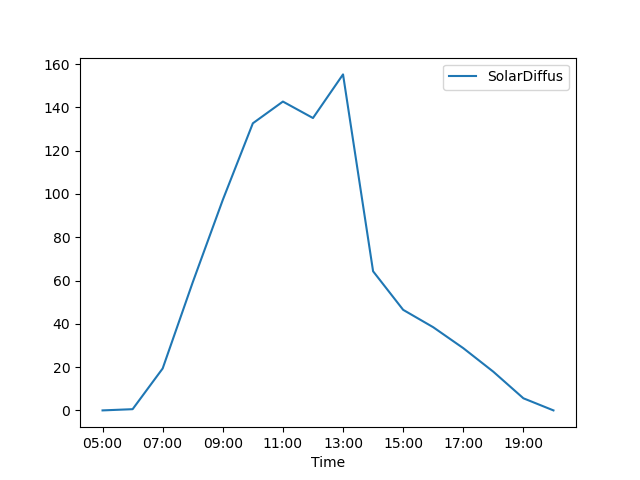
\includegraphics[scale=0.45]{figSolardiffus}
\caption{Évolution de S* et D*.}
\end{center}
\end{figure}
\newpage
En effectuant le calcule sur toute une année et en variant l'inclinaison et l'orientation du panneau nous obtenons ces graphiques pour des albédos différents, ici nous prenons les données du secteur Nord à Gillot:

\begin{figure}[h!]
\begin{center}
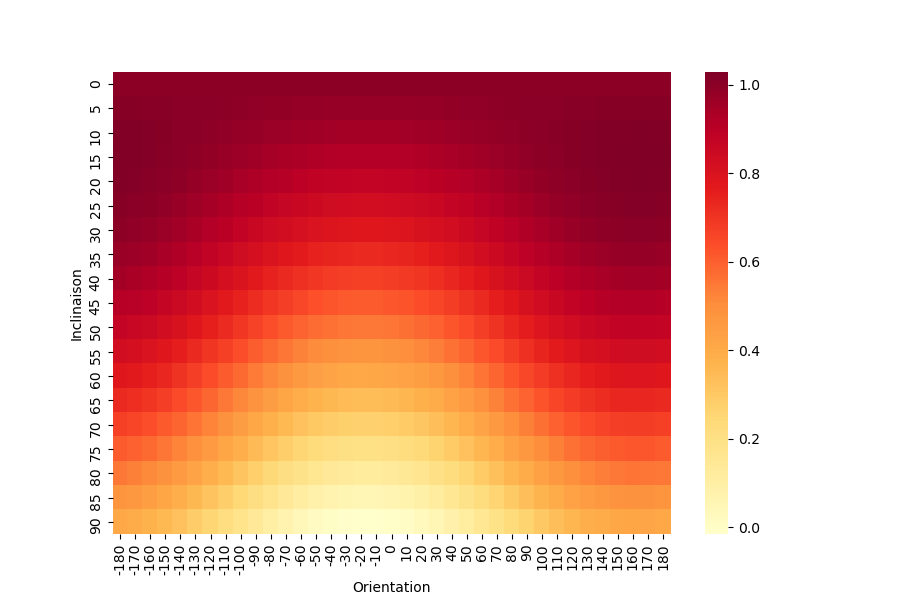
\includegraphics[scale=0.6]{secteurNord}
\caption{Diagramme solaire (albédo = 0,1) pour le secteur Nord.}
\end{center}
\end{figure}

\begin{figure}[h!]
\begin{center}
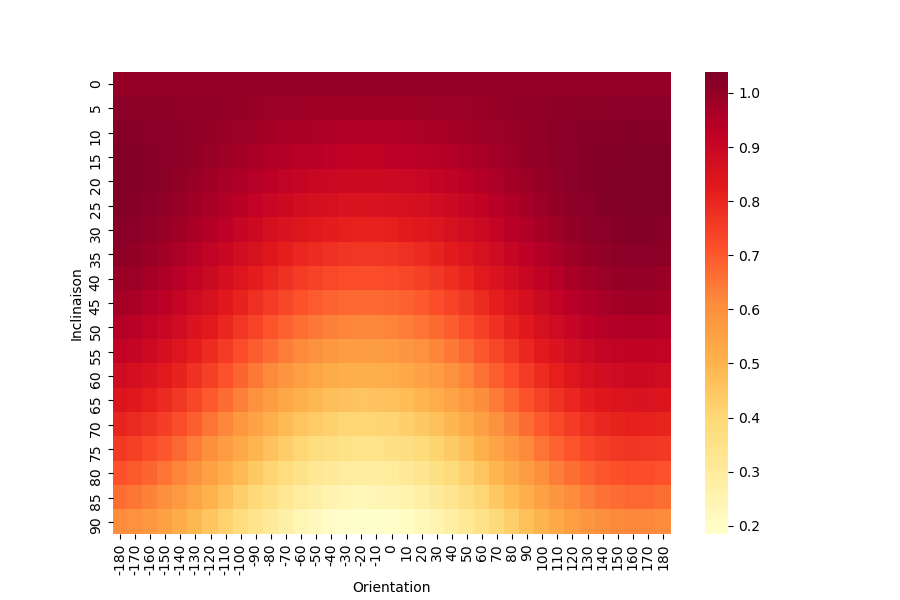
\includegraphics[scale=0.6]{albedo0,5}
\caption{Diagramme solaire (albédo = 0,5) pour le secteur Nord.}
\end{center}
\end{figure}
\newpage

Ainsi que les données suivantes pour les autres secteurs, ces diagrammes sont obtenus avec un albédo égal à 0,1:

\begin{figure}[h!]
\begin{center}
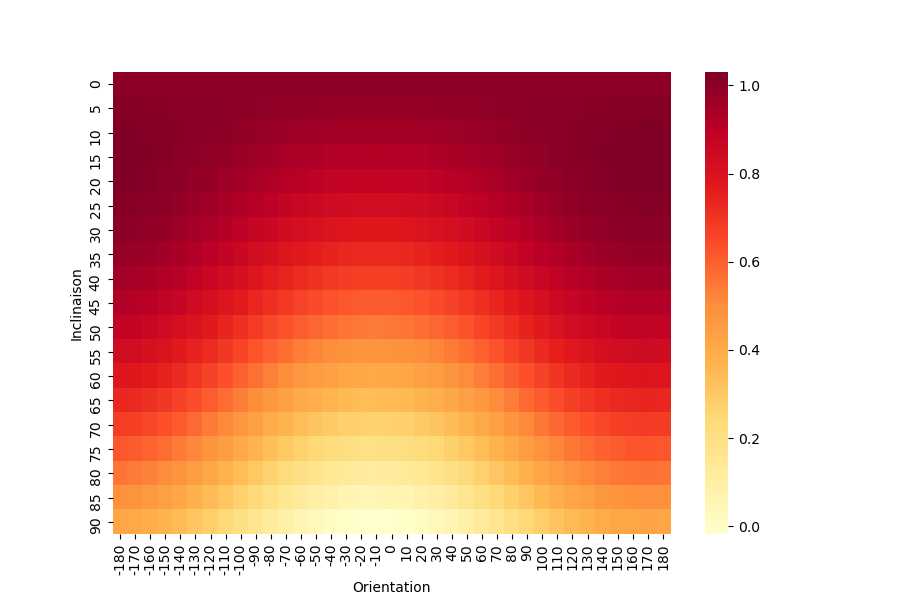
\includegraphics[scale=0.6]{secteurSud}
\caption{Diagramme solaire (albédo = 0,1) pour le secteur Sud.}
\end{center}
\end{figure}

\begin{figure}[h!]
\begin{center}
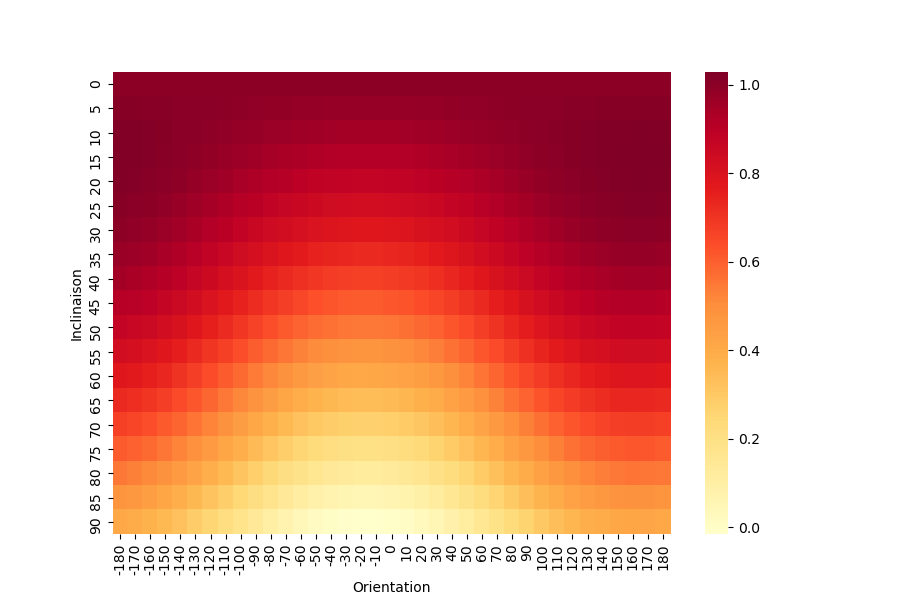
\includegraphics[scale=0.6]{secteurOuest}
\caption{Diagramme solaire (albédo = 0,1) pour le secteur Ouest.}
\end{center}
\end{figure}

\begin{figure}[h]
\begin{center}
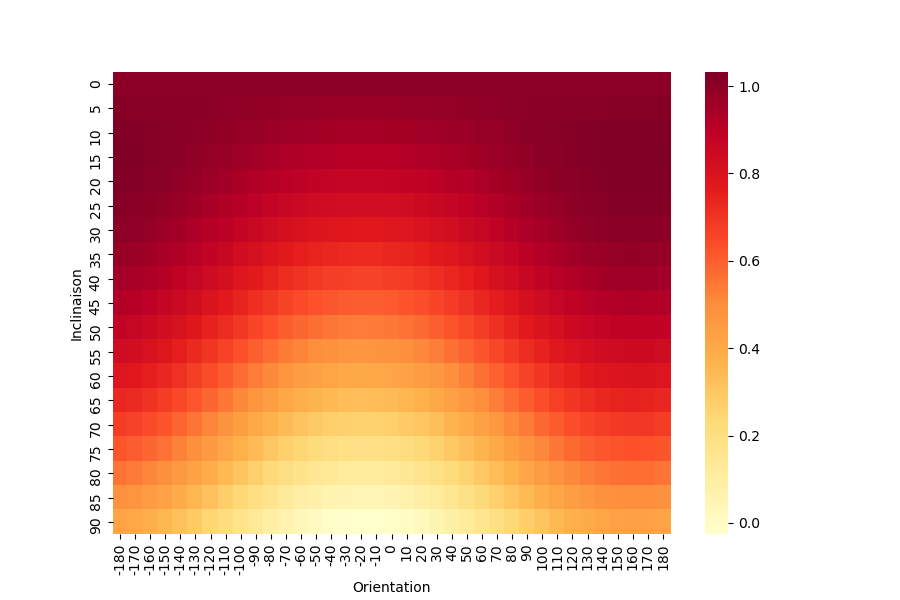
\includegraphics[scale=0.6]{secteurEst}
\caption{Diagramme solaire (albédo = 0,1) pour le secteur Est.}
\end{center}
\end{figure}
\newpage
\begin{figure}[h!]
\begin{center}
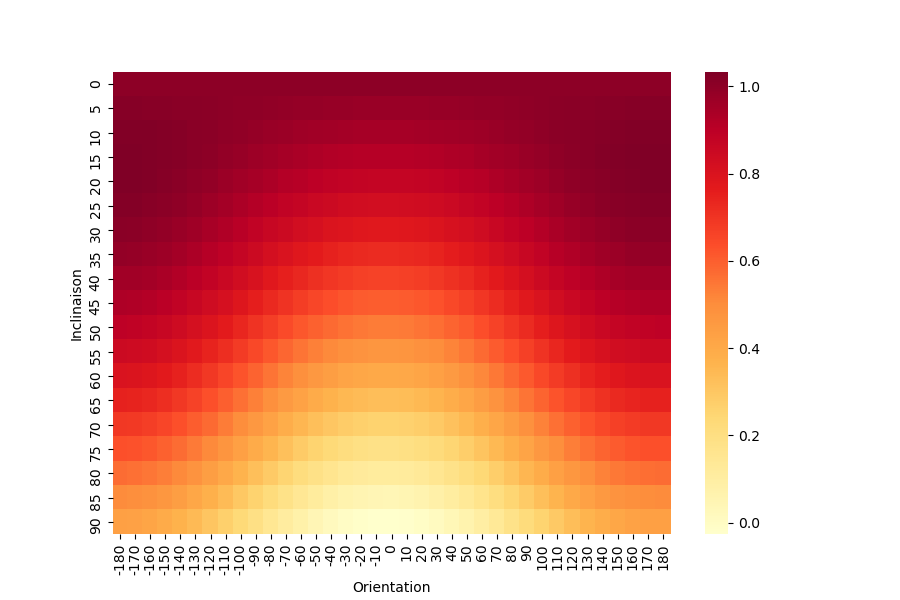
\includegraphics[scale=0.6]{secteurCentre}
\caption{Diagramme solaire (albédo = 0,1) pour le secteur au centre de l'île.}
\end{center}
\end{figure}

\newpage
\section{Discussion}

Nous pouvons voir dans la partie précédente l'évolution de S*, D* et $S_0$; nous pouvons bien constater que D* vaut $\frac{1}{3}$ de $S_0$. Ces données nous montrent l'évolution du rayonnement solaire pendant une journée. Le panneau est fixé pour une inclinaison $i$ et une orientation $\gamma$ égale à un angle de 50°.

Visualiser ces graphiques permet de comprendre le comportement du flux solaire pendant une journée, afin de voir si ces données se rapprochent au mieux de la réalité. Si on observe les 3 graphiques de la \textbf{figure 7} et \textbf{8}, on peut affirmer un pic de flux solaire entre 11h et midi, ce qui nous montre que c'est à ce moment que le soleil donne le maximum de radiation.

On peut se focaliser maintenant sur le calcul du facteur de transposition. Pour rappel, on cherche à visualiser l'angle $i$ et $\gamma$ lorsque le facteur transposition donne sa plus grande valeur. Cela permettra d'optimiser au mieux le panneau solaire. Comme nous pouvons voir sur les diagrammes solaires (\textbf{figure 9 à 14}), la valeur maximale du facteur de transposition n'est pas indiquée. Un programme a été créer pour donner la valeur maximale du facteur de transposition et ainsi que les angles qui lui correspondent :

\begin{figure}[h]
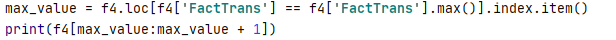
\includegraphics[scale=0.6]{maxvalue}
\end{figure}

Pour le secteur nord, avec un albédo de 0,1 nous obtenons ceci:
\begin{figure}[h]
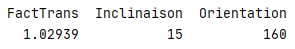
\includegraphics[scale=0.6]{ftigamma}
\end{figure}

Ce que nous pouvons dire des résultats obtenus, c'est que les graphiques semblent trop symétriques par rapport à ce qui nous est donné dans l'\textbf{annexe B}. la valeur maximale du facteur de transposition est loin de ce que l'on peut attendre et ne correspond pas à l'inclinaison et l'orientation qu'ont espérée. Les résultats obtenus ne sont pas concluants malgré leur concordance au niveau visuel. En visualisant toutes les diagrammes solaires, il est difficile les comparer entre eux car ils sont très similaires, si ce n'est qu'un léger décalage dans les zones claires.

L'avancement du stage ne s'arrête qu'à ces résultats, l'objectif de ces deux mois n'a pas pu être atteint dans sa globalité. 
\newpage
	%encadrer un texte
	%\fbox{\begin{minipage}{0.9\textwidth}
   %\textbf{Question 1:} 
	%\end{minipage}}
	%\newpage
	\section*{Conclusion et perspective}
	\addcontentsline{toc}{section}{Conclusion et perspective}
  Ce projet s'oriente principalement sur l'optimisation de l'inclinaison et l'orientation d'un panneau solaire par l'intermédiaire du facteur de transposition. Ce facteur permet d'indiquer l'inclinaison et l'orienter d'un panneau solaire pour qu'il donne le meilleur rendement possible. Il a fallu dans ce projet comprendre théoriquement le comportement du facteur transposition avant d'entamer la programmation, afin de se familiariser avec les différents paramètres et pour avoir plus de clarté lors de l'étude.
  
  L'objectif de ce stage a été atteint à 80\% selon l'encadrant. Le projet n'a pas pu être terminé, mais il y a eu tout de même des résultats à interpréter.
  
  Les compétences acquises lors de ce stage sont liées à l'utilisation d'un logiciel de programmation, à la recherche et à la lecture des données solaire, et de savoir construire un algorithme à partir de différentes équations.
  
  Ce stage m'a permis de me familiariser avec un logiciel que je connaissais peu et que je n'osais pas vraiment l'utiliser. J'ai pu expérimenter davantage sur le fait de travailler en autonomie et acquérir plus de connaissances que ça soit dans la recherche ou la lecture des données solaire.
  
	\newpage
	
\listoffigures
\newpage

\appendix
\chapter{Calcul de flux solaire.}
\begin{figure}[h!]
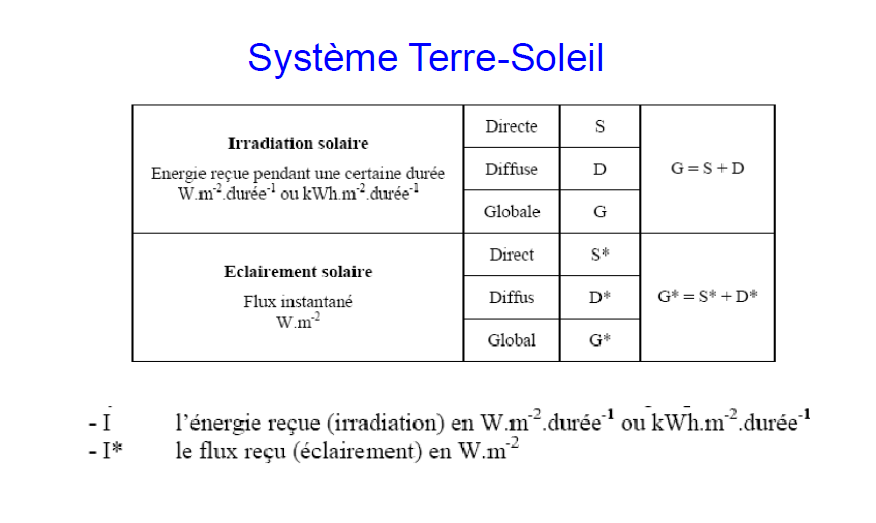
\includegraphics[scale=0.7]{RoyGlo}
\end{figure}
\chapter{Diagramme albédo de référence pour un albédo de 0.1 et 0.5.}
\begin{figure}[h!]
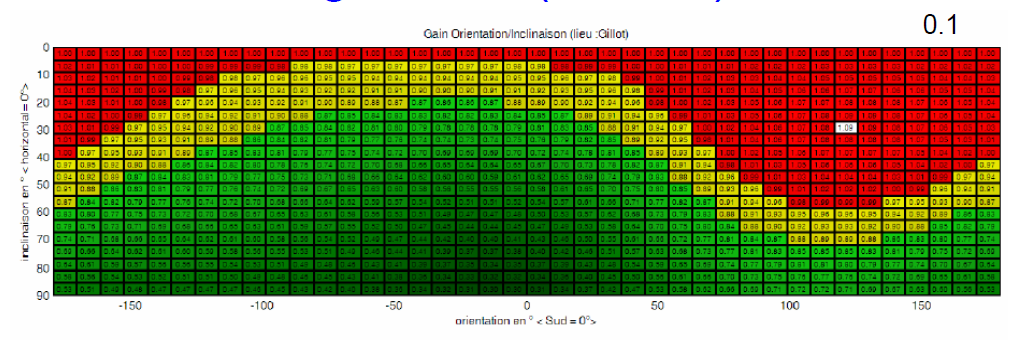
\includegraphics[scale=0.6]{diagramme1}
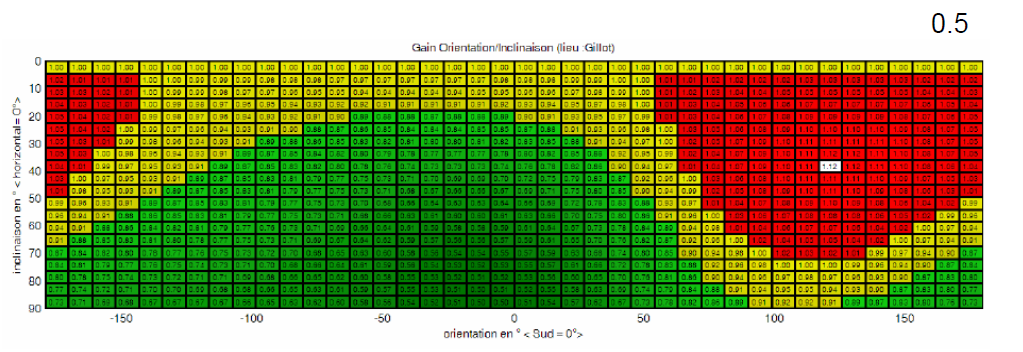
\includegraphics[scale=0.6]{diagramme2}
\end{figure}
\chapter{Codage du facteur de transposition.}
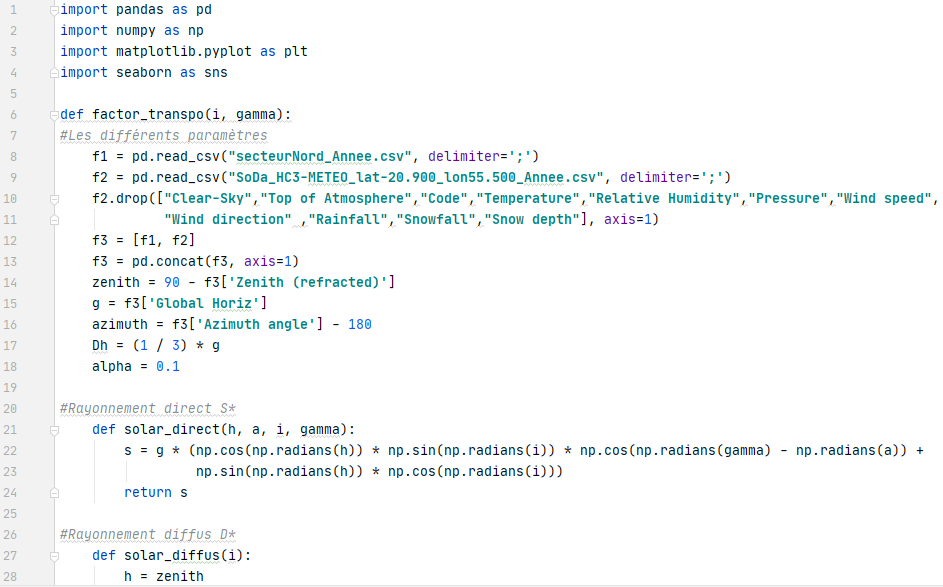
\includegraphics[scale=0.5]{prog1}
\newline
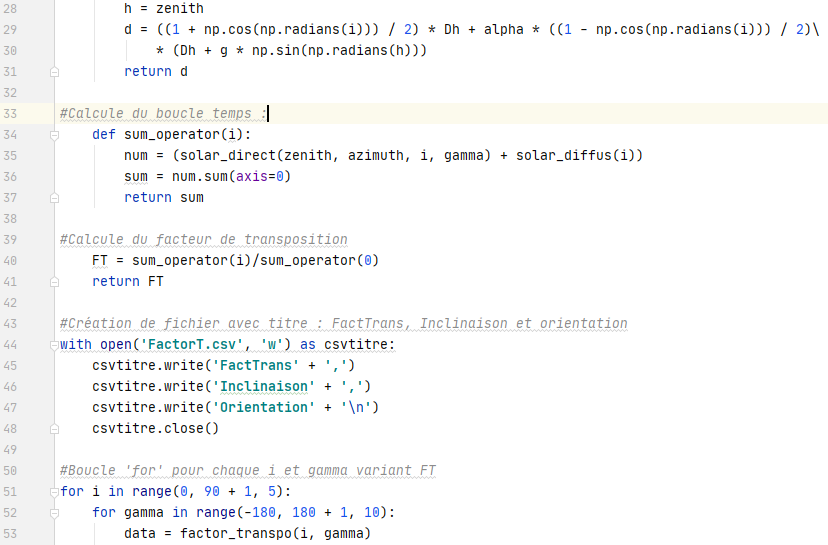
\includegraphics[scale=0.5]{prog2}
\newpage
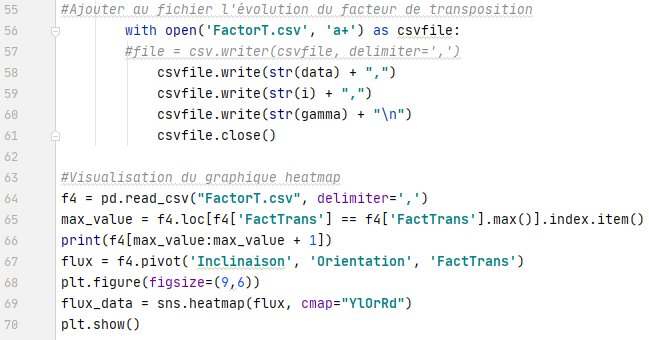
\includegraphics[scale=0.5]{prog3}
\end{document}

